\documentclass[twocolumn]{amsart}
\usepackage{tikz}

\begin{document}

\section{I, Robot}

This summer I had the pleasure to work with three very gifted students on an ambitious project to code our NAO robot\footnote{\tt http://www.aldebaran.com/en/humanoid-robot/nao-robot}, \emph{Astro}.  The first goal was to have Astro perform some fun autonomous tasks: playing word games, moving around obstacle courses picking objects, or reading music from a partiture and playing it for us.  We are even planing to write code that will allow Astro to look for a set of chess pieces, place them all on a board in the right position, and physically play against us.

One of the advantages of a NAO robot is that it requires very little knowledge of actual programming to code it.  The students took a 13-hour online beginner course on {\tt python}, and in about one week they were able to control most of Astro's basic functionality.  This allowed them to focus on the \emph{mathematics} alone.   In that sense, they had to spend some time reviewing their background geometry and algebra: sequences, lines and circles, systems of linear equations, polynomials and their roots, nonlinear equations and their solutions, polynomial interpolation, etc.  They also needed some Calculus (nothing more complicated than derivatives and tangent lines), and some basic statistics.

This allowed them right away to solve some fun problems in obstacle avoidance, for example.  

\begin{figure}[h!]
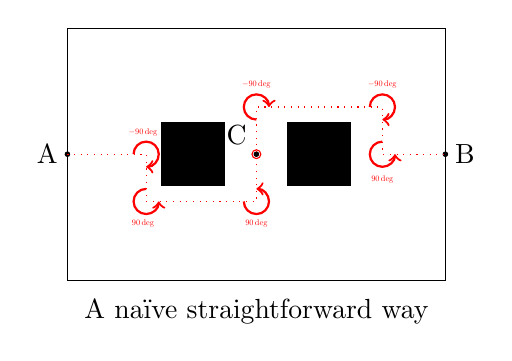
\begin{tikzpicture}[scale=0.4]
\draw (0,0) rectangle (12cm, 8cm);
\filldraw (0cm, 4cm) circle (2pt) node[left]{A};
\filldraw (12cm, 4cm) circle (2pt) node[right]{B};
\filldraw (6cm, 4cm) circle (2pt) node[anchor=south east]{C};
\draw[red] (6cm, 4cm) circle (4pt);
\filldraw (3cm, 3cm) rectangle (5cm,5cm);
\filldraw (7cm, 3cm) rectangle (9cm,5cm);
\draw[red, dotted] (0, 4) -- (2.5, 4) -- (2.5, 2.5) -- (6, 2.5) -- (6, 5.5) -- (10, 5.5) -- (10, 4) -- (12, 4);
\draw[->, red, thick] (2.1, 4) arc[x radius=0.4cm, y radius =.4cm, start angle=180, end angle=-90];
\draw[red] (2.4, 4.7) node[scale=0.3]{$-90\deg$};
\draw[->, red, thick] (2.5, 2.9) arc[x radius=0.4cm, y radius =.4cm, start angle=90, end angle=360];
\draw[red] (2.4, 1.8) node[scale=0.3]{$90\deg$};
\draw[->, red, thick] (5.6, 2.5) arc[x radius=0.4cm, y radius =.4cm, start angle=-180, end angle=90];
\draw[red] (6, 1.8) node[scale=0.3]{$90\deg$};
\draw[->, red, thick] (6, 5.1) arc[x radius=0.4cm, y radius =.4cm, start angle=270, end angle=0];
\draw[red] (6, 6.2) node[scale=0.3]{$-90\deg$};
\draw[->, red, thick] (9.6, 5.5) arc[x radius=0.4cm, y radius =.4cm, start angle=180, end angle=-90];
\draw[red] (10, 6.2) node[scale=0.3]{$-90\deg$};
\draw[->, red, thick] (10, 4.4) arc[x radius=0.4cm, y radius =.4cm, start angle=90, end angle=360];
\draw[red] (10, 3.2) node[scale=0.3]{$90\deg$};

\draw (6cm, -1cm) node{A na\"\i ve straightforward way};
\end{tikzpicture}

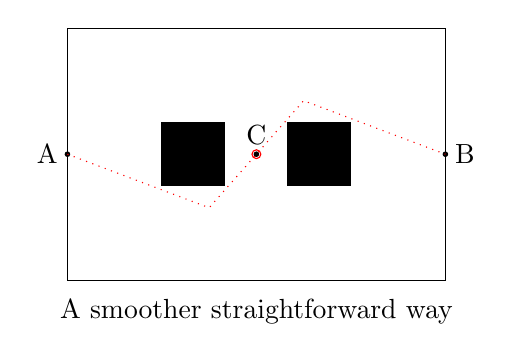
\begin{tikzpicture}[scale=0.4]
\draw (0,0) rectangle (12cm, 8cm);
\filldraw (0cm, 4cm) circle (2pt) node[left]{A};
\filldraw (12cm, 4cm) circle (2pt) node[right]{B};
\filldraw (6cm, 4cm) circle (2pt) node[above]{C};
\draw[red] (6cm, 4cm) circle (4pt);
\filldraw (3cm, 3cm) rectangle (5cm,5cm);
\filldraw (7cm, 3cm) rectangle (9cm,5cm);
\draw[red, dotted] (0,4) -- (4.5,2.3) -- (7.5, 5.7) -- (12,4);
\draw (6cm, -1cm) node{A smoother straightforward way};
\end{tikzpicture}

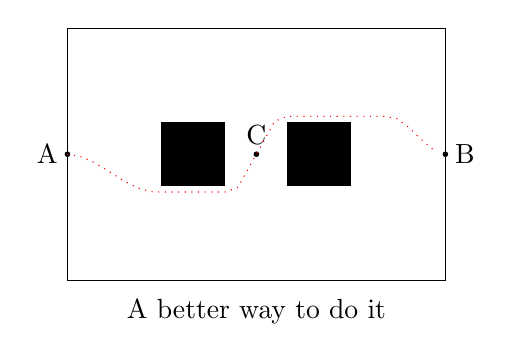
\begin{tikzpicture}[scale=0.4]
\draw (0,0) rectangle (12cm, 8cm);
\filldraw (0cm, 4cm) circle (2pt) node[left]{A};
\filldraw (12cm, 4cm) circle (2pt) node[right]{B};
\filldraw (6cm, 4cm) circle (2pt) node[above]{C};
\filldraw (3cm, 3cm) rectangle (5cm,5cm);
\filldraw (7cm, 3cm) rectangle (9cm,5cm);
\draw[red, dotted] (0.0, 4.0) -- (0.387096774194, 3.93753567737) -- (0.774193548387, 3.77550893186) -- (1.16129032258, 3.55196909705) -- (1.54838709677, 3.30496550654) -- (1.93548387097, 3.0725474939) -- (2.32258064516, 2.89276439271) -- (2.70967741935, 2.80366553657) -- (3.09677419355, 2.8) -- (3.48387096774, 2.8) -- (3.87096774194, 2.8) -- (4.25806451613, 2.8) -- (4.64516129032, 2.8) -- (5.03225806452, 2.8) -- (5.41935483871, 2.95569970797) -- (5.8064516129, 3.65643147259) -- (6.1935483871, 4.34356852741) -- (6.58064516129, 5.04430029203) -- (6.96774193548, 5.2) -- (7.35483870968, 5.2) -- (7.74193548387, 5.2) -- (8.12903225806, 5.2) -- (8.51612903226, 5.2) -- (8.90322580645, 5.2) -- (9.29032258065, 5.2) -- (9.67741935484, 5.2) -- (10.064516129, 5.2) -- (10.4516129032, 5.13621190591) -- (10.8387096774, 4.85394917928) -- (11.2258064516, 4.47501296066) -- (11.6129032258, 4.14262323819);
(12.0, 4.0) -- 
\draw (6cm, -1cm) node{A better way to do it};
\end{tikzpicture}
\caption{Simple obstacle race.  Go from $A$ to $B$, picking and object at $C$ in the way.}
\end{figure}

The diagram shows two ways in which the robot solves the obstacle race. The \emph{easy} way is by walking forward in a fixed direction, then stopping, rotating in place to look in a new direction, and walk straight again.  This is efficient, but too robot-like.   We can do much better: by employing simple interpolation techniques, the robot learns to take a smoother approach, reminiscent of how humans walk.


\end{document}